
\documentclass[12pt]{article}
\usepackage{fancyhdr}
\usepackage[margin=1.05in]{geometry}
\usepackage{alltt}
\usepackage{xcolor}
\usepackage[utf8]{inputenc}
\usepackage{pgfplots}
\usepackage{tikz}
\usepackage{etoc}
\usepackage[hidelinks]{hyperref}
\usepackage{amsmath}
\usepackage{amssymb}
\usepackage{biblatex}
\usepackage{cancel}
\usepackage{breqn}
\usepackage[euler]{textgreek}
\usepackage{graphicx}
\usepackage{subfig}
\usepackage{float}
\usepackage[labelfont=bf, margin=1cm]{caption}
\usepackage{listings}
\usepackage{color}
\graphicspath{{/home/user/Desktop/secpred/Project-MTLS/Plots}}
\definecolor{dkgreen}{rgb}{0,0.6,0}
\definecolor{gray}{rgb}{0.5,0.5,0.5}
\definecolor{red}{rgb}{0.8,0,0}
\renewcommand{\baselinestretch}{1.0}
\DeclareMathOperator*{\argmin}{arg\,min\:}


\begin{document}

\begin{titlepage}
\begin{center}

\textsc{\LARGE Project in Molecular Life Science} \\[0.5cm]

\emph{ Stockholm University, Spring Term 2018 \\ by: Maryia Ropat } \\[3cm]

{\Huge \bfseries Predicting 3-state Protein Secondary Structure from Sequence \\ and PSSM Profiles} \\[7cm]

\vfill

\end{center}
\end{titlepage}

\newpage

\tableofcontents

\vfill

\newpage


\section{Background}

\subsection*{Protein secondary structure assignment}

As we may know, protein secondary structure is either assigned manually by crystallographers, or automatically by assignment algorithms such as DSSP, STRIDE, or DEFINE. 
The DSSP assignment method uses information about intra-backbone hydrogen bonds, and STRIDE uses the previously mentioned criteria, in addition to dihedral angle potentials. In general, DSSP will assign a larger fraction of helical regions compared to STRIDE, and both will under-assign $ \pi $-helices. DSSP and STRIDE perform similarly well on manually assigned data, and there is a 95\% overlap in consensus between them.
Despite these methods being considered equivalent, DSSP assignment is much more commonly used for training new predictors. This preference is rarely discussed, but DSSP is older and more established, and the helical length differences may lead to DSSP-trained predictors performing slightly better at certain tasks\cite{2}.
\subsection{State reduction}

Both DSSP and STRIDE tend to output 8-state secondary structure assignments\cite{5}\\

\begin{alltt} 
  H	    Alpha helix
  G	    3-10 helix
  I	    PI-helix
  E	    Extended conformation
  B, b  Isolated bridge
  T	    Turn
  C	    Coil (none of the above)
          
\end{alltt}

\noindent Prediction of 8-state secondary structure is harder, and sometimes quick and easy generalizations are needed to determine the general protein architecture, in order to easier classify them into groups and study similarities. There are three different principles by which the assigned 8-state secondary structure is reduced to 3-state secondary stricture:\\
\begin{alltt}
	  A: E,B-> E; G,H-> H; rest is coil
	  B: E  -> E;   H-> H; rest is coil,including short segments of H and E
	  C: E  -> E;   H-> H; 4xG adjacent to H -> H,rest is coil
	  
\end{alltt}	    
Different researchers prefer to reduce using different principles: PhD method used A, while PREDATOR uses C. It becomes difficult to compare performance of methods, when different reduction schemes are used, and overall, A is considered the harshest metric, assigning more structures as “regular structures”, while C relaxes the definition, assigning more structures with no periodicity to coil. In general, accuracy of most methods improves on data reduced by scheme C, but it is up to the researcher to determine which approach suits their experiment best\cite{5}. Bottom line is, this should be kept in mind when discussing and evaluating state of the art and performance of models in the future - as there is no unified standard, many of the performance numbers we see could be generated using different definitions and metrics. 

\subsection{State-of-the-art predictors}

For many years, there have been few major breakthroughs in secondary structure prediction. This has changed with the increasing popularity of deep learning and novel methods appearing as a result.  One of the currently highest performing predictors is  the DNN-based SSREDN\cite{4} predicting  92.8\% -94\%, which, to put in perspective, is almost as high as the consensus between existing assignment methods DSSP and STRIDE.
Among the long-lived state-of-the art predictors are ANN-based Jpred (Q3 of 82\%) and PSIPRED\cite{6} (Q3 of 81\%). For SVM predictors, highest performance, using evolutionary information, tops off at 73.5\%, with dual-layer SVM methods such as PMSVM\cite{1} reaching the Q3 of 75\% and SOV of 80\%.



\section{Processing the data}


\subsection{Training dataset}

For this task, it was suggested to use a training dataset of 396 sequences with assigned structures. Upon investigation, it was determined that the structures in the dataset were reduced by the strictest criteria A. 
To come to that conclusion, we examined the original 8-state structure assignment for a sample protein from original dataset, and determined which reduction scheme was performed:
\begin{alltt} 

	  C: If there are G regions adjacent to H, and they are reduced to H
	  A: If B is assigned to E(or S in our dataset)
	  B: If none of the above                                           
	   
\end{alltt}	
There was also a fair amount of redundancy within the dataset, with several chains originating from the same entry and having a high degree of sequence similarity, but alternative structure assignments. Such data will understandably influence difficulty of training and quality of the classifier. To find and eliminate such redundancies, we can run a longest substring query on sequences in our dataset, and eliminate sequences above a certain threshold from training data. 
For the dataset containing 396 entries, this might take a long time, so a dynamic solution is recommended. Our threshold for elimination has been 15, which equals to the smallest sliding window size used for our training (more on which we discuss in later sections). This ensures that our input vectors will always be unique.
In total, we found 26 such sequences in our dataset, and upon elimination of those sequences, the final performance scores and training times of our predictor saw a marginal, but welcome improvement. 


\subsection{Creating an input vector}


Input format
Many classifiers supported by scikit-learn have a similar input format for our training data.\\

\indent X =  two-dimensional array with dimensions [number of features, feature vectors]\\
\indent   y  =  one-dimensional array of size [number of features]\\

\noindent Inputs are generated by associating a region in the sequence with a structural class by means of sliding windows: \\

   Sequence:    MNTPEH\colorbox{pink}{MTAVVQRYVAALNAG}DLDGIV    $ \longrightarrow $ X, features\\

   Structure: CCCHHHHHHHHHH\colorbox{red}{H}HHHHHHCCHHHH  $ \longrightarrow $ y, classes\\
   

\subsubsection{Sparse and dense vectors}

Before introducing to our algorithm, we have to transform our sequence features into a numeric format. 
Input vectors utilized in machine learning are often distinguished by being dense or sparse. A dense vector contains members which are mostly non-zeros. A sparse vector contains members that are mostly zeros and some non-zeros. Generally, dense data is harder to process and store, which leads to longer training times and higher RAM consumption.\\ 

\noindent \textbf{Example of dense vector:}

\begin{alltt} 
	([ 0.1,   0.2,   0.3,   0.4,   0.5,   0.6,   0.7,   0.8,   0.9,   1.0])
	
\end{alltt} 
	\textbf{Example of sparse vector:}
\begin{alltt} 
	([ 0.,    0.,    0.,    0.,    0.,    0.,    0.,    0.,    0.,    1.0.])
	
\end{alltt} 

\noindent The simplest way to encode our data into feature vectors is by using OneHotEncoder included scikit-learn, or by encoding it manually by assigning a member of identity matrix to each amino-acid. Both approaches will produce feature vectors containing sparse data, which can be used to input features into our algirhithm of choice. \\
\newpage


\subsection{Using PSSM or BLOSUM/PAM to represent features}

Similarly, we could encode our feature vectors using the evolutionary information stored in BLOSUM or PAM matrices, or with data generated by PSI-BLAST. 
PSI-BLAST outputs two types of matrices: substitution matrix and frequency matrix. The frequency matrix contains less information, but is easy to represent in sparse vectors, while the substitution matrix carries more information, but also leads to longer training time and and more complicated models.
The substitution matrix gained from PSI-BLAST outputs or BLOSUM/PAM matrices can be transformed with the sigmoid function\cite{3}, which places values within the range of 0 and 1, where zeros are found at 0.5 mark. As suggested by the name, the biggest value separation lies around the 0.5 mark, and the more extreme values would appear much closer after transformation. \\\\

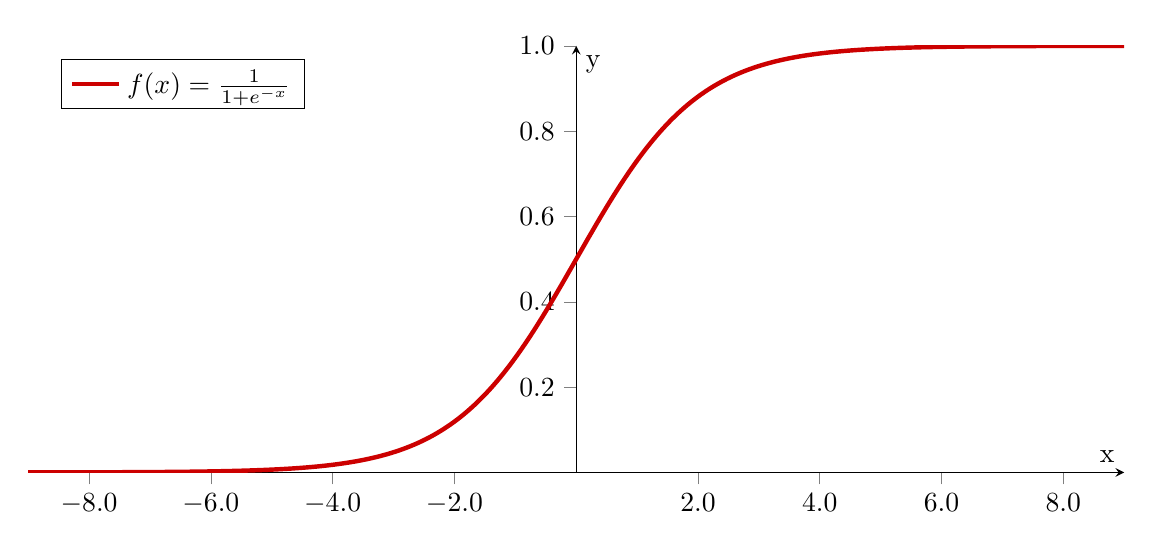
\begin{tikzpicture}
    \begin{axis}[
    	legend pos=north west,
        axis x line=middle,
        axis y line=middle,
        x tick label style={/pgf/number format/fixed,
                            /pgf/number format/fixed zerofill,
                            /pgf/number format/precision=1},
        y tick label style={/pgf/number format/fixed,
                            /pgf/number format/fixed zerofill,
                            /pgf/number format/precision=1},
        width=15.5cm,
        height=7cm,
        grid style={dashed, gray!30},
        xmin=-9,  
        xmax= 9,
        ymin= 0, 
        ymax= 1,
        xlabel=x,
        ylabel=y,
        tick align=outside,
        enlargelimits=false]
      \addplot[domain=-9:9, red, ultra thick,samples=500] {1/(1+exp(-x))};
      \addlegendentry{$f(x)=\frac{1}{1+e^{-x}}$}
    \end{axis}
\end{tikzpicture}\\

\noindent This transformation populates the vectors with dense data. For the sake of improvement of training times and  reducing the model size, we also set every resulting\\ value $ < $ 0.1 to 0, which might result in only a marginal decrease in accuracy of some predictors, but also leads a decrease in training times and model save size. Interestingly, Decision Trees will  perform much better due to this final transformation, which shows that reducing the complexity of the data could sometimes go a long way in improving predictor performance. \\
Similarly, this transformation can also be performed on BLOSUM or PAM substitution matrices, which may lead to a boost in the  performance of a predictor when only sequence information is available.\\
Below, we compare performance of two most common algorhithms when inputs are encoded with BLOSUM matrix information and ordinary one-hot encoding.
\newpage
\noindent We have found (and verified several times) that using BLOSUM substitution matrix to encode sequence information had absolutely no effect on perfromance of LinearSVC:

\begin{figure}[H]
\hspace*{-0.5in}
\includegraphics[scale=0.5]{../Plots/linsvc_blo.png}
\hspace*{-0.75in} 
\includegraphics[scale=0.5]{../Plots/linsvc_ohe.png}
\caption{Comparison of LinearSVC performance with sequence data encoded by BLOSUM and one-hot encoding}
\end{figure} 


\noindent This suggests that the evolutionary information based on amino-acid frequencies may already be captured by the linear kernel. \\
\noindent On the other hand, performance of Random Forests was greatly improved by this addition, by a margin that is larger than what can be attributed to variance:

\begin{figure}[H]
\hspace*{-0.5in}
\includegraphics[scale=0.5]{../Plots/RFBLOxval.png} 
\hspace*{-0.75in}
\includegraphics[scale=0.5]{../Plots/RFohexval.png} 
\caption{Comparison of Random Forest performance with sequence data encoded by BLOSUM and one-hot encoding}
\end{figure}
\newpage

\section{Training and testing}

\subsection{Creating naive dataset for testing}

Since STRIDE assignments are rarely used for training predictors,  and most servers provide only reference datasets, we decided to construct out own naive dataset for final testing. 
PDBe was queried with the following terms 
\begin{alltt} 
   CATH class    : "Alpha Beta"
   Assembly comp : "protein structure"
   Assembly type : monomer
   Release year  : [2000 TO 2005]
   Superkingdom  : Eukaryota
   Resolution    : [2.5 TO 3]
\end{alltt} 
We decided on class Alpha Beta as the members would be somewhat representative of our training set. We also have chosen to see monomers only, even if that was not true for our training data, but would simplify further processing and result in larger average chain size. The resulting list has been verified for homology (using the longest common substring algorithm) within itself and with training set, and has a roughly same proportion of C, H and S elements as the one used in training. This dataset, besides the cross-validation scoring, will be used to evaluate the final performance of our predictors. If needed, any number of entries could be used for testing, but for the purpose of the project, we will start with 50.\\
To get STRIDE assignments, we download an archive from \emph{http://www.rcsb.org/} containing all PDB files for our new dataset. While STRIDE already has pre-assigned a lot of the PDB entries, at the time of this project, it was no loger possible to fetch assignments from multiple entries at once. Fortunately, they still provide access to many resources at \emph{ftp.ebi.ac.uk}, including installation files needed to run the service locally, and a large archive of preassigned PDB entries up to release year ~2000.
As our testing dataset PDB entries contains multiple chain information, we settle on extracting only chain A assignments for the sake of creating a heterogenic testing sample.



\subsection{Sliding window size}

When training a model, the first metric to be evaluated and tweaked is the sliding window size. With every classifier, the performance at default settings was initially tested on a range of sliding windows from size 5 to 25.\\
For many classifiers, trained on input of every type of encoding, the prediction accuracy would increase until window size 21 is reached, upon which it would taper off or decrease.
Exceptions to this have been decision trees and unoptimized  fandom forests, which peak at window size of 15 residues. This observation contradicts the common scientific consensus of the optimal window size of 15.\\
\newpage
\noindent Since most predictors described in the literature have been trained on DSSP data, we compared the effect of sliding window size on cross-validation scores between DSSP and STRIDE.
\begin{figure}[H]
\hspace*{-0.3in}
\includegraphics[scale=0.9]{../Plots/Windowsize.png}
\caption{Comparison of sliding window sizes and their effect on LinearSVC performance (sequence only, BLOSUM encoded)}
\end{figure}

\noindent We hoped to see a difference of optimum window size for data assigned by the two methods, but found no such relationship. However, the overall performance of LinearSVC was better over all window sizes for DSSP, which might hint to why this assignment method is preferred for training most predictor models. \\
Still, this plot suggests that relevant information might be gained from residues which are 10 positions away, as opposed to 7, as we can see a consistent peak followed by a plateu for both DSSP and STRIDE data.  


\subsection{Support Vector Machines}

SVMs are a very powerful tool for classification, and when first introduced into the research space, were very successful at secondary structure prediction. 
LinearSVC and SVM.SVC predictors both separate data using the linear kernel. However, LinearSVC trains much faster, since the training time increases only linearly with added vector dimensions, as opposed to exponential with SVC(linear), while providing a similar result, which makes it our preferred classifier for linear kernel.\\
While the unoptimized performance of LinearSVC was initially fairly good, titrating over the values of C between 0.5 to 2.0 and all available parameters of "loss" and "hinge", as well as adjusting class balance only lead to mean accuracy decrease on cross-validated sets. This leads us to conclude that default (C=1, l2, hinge=squared) LinearSVC can generealize well on our data, but has no optimization potential, and might not be an optimal kernel for our data.\\
SVMs with kernel “rbf”, while already experimentally proven to be excellent at secondary structure classification\cite{1} \cite{3}, take a very long time to train. In the timespan of this project, it was implausible to optimize and evaluate over a wide range of values and window sizes, and so we decided to apply and verify performance of the kernel parameters used in a published article for PMSVM predictor: \emph{window size} = 15; $\lambda$=0.05, C=2.3. We also trained a model with the same parameters, except for the window size 21 (shown on the right). \\
\begin{figure}[H]
\hspace*{-0.75in}
\includegraphics[scale=0.65]{../Plots/rbf_stride_15.png} 
\hspace*{-0.8in}
\includegraphics[scale=0.65]{../Plots/rbf_stride.png} 
\caption{Comparison of performance: RBF SVM of window sizes 15 and 21}
\end{figure}
\noindent Due to very long training times of these models, and the fact that we did not find these parameters ourselves, we did not test the performance on cross-validated sets, and these scores indicate the performance on our testing dataset of 50 proteins.\\[0.1cm]
As we can see from the scores, SVM with this kernel, trained on our data, performs even better on our test set than reported performance on the GOR set in PMSVM article\cite{1}
\noindent The overall perfromance of the model is improved with the addition of information at 10 residue distance, but there is a trade-off: our model is now better at correctly identifying coil structures and worse at identifying $ \beta $-sheets. Whetehr this is a true performance increase is arguable, since this  increased recall for the coil class, which is more abundant in training and testing data. 


\subsection{Random Forest Classification}

Random forests are trained as an enseble of decision trees. The trees are trained separately after initially randomily dividing the datapoints among themselves, while still maintaining global class proportions. Subsequently, the trees are grown and split at each node based on a random set of selected features. When used for prediction, trees will produce a (democratic) jury decision in order to classify the data. \\
Due to the randomness of the training process, Random Forests will produce a different model at each new iteration with the same settings. To successfully evaluate effect of optimizations on the model, it is recommended to select and use the same seed in order to reduce the variance between runs.\\
Random forests also have a built-in attribute \textbf{{\_}oob{\_}score} which can be used similarl to cross-valiation scores to estimate performance. Due to the architecture of the algorhithm, there are always some datapoints which did not contribute to splitting at other nodes, and these features are then used in order to produce this quality assessment score. Since some features are related and dependent on one another, this metric is not completely impartial, especially when using parameter \textbf{min{\_}impurity{\_}decrease} to optimize our model.\\
When it comes to optimization of random forests, one of the most powerful parameters is the number of trees \textbf{(or n{\_}estimators)} participating in jury decision.  Generally, higher number of trees produces higher  accuracy and lower variance, up to a certain point, which depends on the size of the dataset and our other training parameters. \\
Parameter \textbf{max{\_}features} is also very important for optimization, as it denotes how many features are evaluated at each split. \\
As the Random Forests are known to overfit, parameters like \textbf{min{\_}impurity{\_}decrease} and \textbf{min{\_}samples{\_}leaf} can be important for optimization.\\ Specifically, \textbf{min{\_}impurity{\_}decrease} has been one of the most interesting parameters to manipulate, as helps the algithithm to generalize on correlated data (and sliding window data contains many correlated features because of helical and sheet periodicity).
Our final optimized random forest model has the following parameters:\\[0.5cm]
\indent \textbf{n{\_}estimators = 1600}\\
\indent \textbf{max{\_}features = 35}\\
\indent \textbf{min{\_}impurity{\_}decrease = 0.000015}\\
\indent \textbf{min{\_}samples{\_}leaf = 3}\\

\noindent Increasing number of trees past this point point did not have any positive effect on cross-validation accuracy, while other features were carefully titrated one-by-one in the order they are listed above (as opposed to grid search approach).\\ When the paremeter performance reached local maximum, which was evaluated by oob and cross-validation scores, we moved on to the next one, starting from the default values suggested by scikit-learn. We did not optimize more parameters past that point, as the performance was optimized around the default values, and tweaking would no longer have a positive impact on the performance. This approach might lead to missing out on some combinations of parameters that perform better otherwise, but takes a lot less time while producing a reasonable result. \\
\begin{figure}[H]
\hspace*{-0.6in}
\includegraphics[scale=0.5]{../Plots/xval_forest.png}
\hspace*{-0.6in} 
\includegraphics[scale=0.5]{../Plots/forest50.png} 
\caption{Comparison of Random Forest performance on cross-validated set versus testing dataset}
\end{figure}

\noindent As we can see from the graphs, our model still does not generalize very well and struggles with distinguishing coil/sheet, especially on the test set of 50 proteins. Random forests were in general struggling the most with imbalance of Coil/Sheet classification performances: when optimizing for precision/recall ratio, we tried to strike a healthy balance as the recall metric for coil would correlate with precision metric for sheet.



\subsection{Decision Trees}
The underlying principle behind the Decision Frees is similar to Random Forests, except the singular Decision Tree will be trained on the entire dataset. Like with random forests, we could specify our favorite favorite seed number for consistency of evaluation. As the tree is trained on all features at once, it will generalize heavily and be very susceptible to overfitting.\\
Decision Trees can be visualized, and are excellent in cases when you would like to extract the rules steering the decision process in classification. Unfortunately for us, for our research question, these rules are not binary.\\ Decision Trees are not very good at dealing with complex multidimensional, and dense data. As mentioned earlier, reducing complexity of our data by treating every value of substitution matrix that is smaller than -4 as -$\infty$ could boost the perfromance score of our Tree predictor by 1.5\%! Decision Trees have also shown to perform the best at window size of 15 as opposed to 21.\\
\newpage
\noindent We also verified whether we could extend the "reduce and simplify" approach even further, and see an even better performance with frequency matrix data (instead of substitution), but that was not the case.
\begin{figure}[H]
\hspace*{-0.6in}
\includegraphics[scale=0.65]{../Plots/tree_vxl.png} 
\hspace*{-0.6in}
\includegraphics[scale=0.65]{../Plots/tree_stride.png}
\caption{Comparison of performances of decision tree classifier on cross-validation sets versus testing set}
\end{figure}

\noindent As shown above, our final model performs even better on testing set, than cross-validated set. This might indicate a few things: either that it is a weak or poorly optimized model, and can get a better result by chance; it might also generalize best on patterns which are more abundant in test set. Overall, we believe simple decision trees are not a suitable classifier for our problem, the drawbacks and tuning is similar to random forests for our data, but with even more class imbalance and without the compensation for randomness and bias.
\subsubsection{AdaBoost}

We also evaluated the potential performance of Decision Trees as a part of another ensemble structure. AdaBoost algothithm will fit a lot of weak learners (like our Decision Tree, but others can be selected), and learn from the data over multiple iterations. In each iteration, sample weights will be readjusted to ephasize the ones guessed incorrectly in previous iterations.  AdaBoost is similar to Random Forests, in a way that consensus is gained by jury decision, but AdaBoost will weigh those votes differently  depending on how they performed during training process.\\
\begin{figure}[H]
\hspace*{-0.6in}
\includegraphics[scale=0.51]{../Plots/xval_adaboost.png} 
\hspace*{-0.6in}
\includegraphics[scale=0.65]{../Plots/adaboost_stride.png} 
\caption{Comparison of out-of-the-bag AdaBoost performance on cross-validated and testing sets}
\end{figure}

\noindent Our AdaBoost model performs best at window size 21, and we can note that compared to Random Forests and simple Decision trees, this predictor will identify a much larger proportion of $\beta$-sheets correctly, and overall have the least amount of class bias and a precision/recall ratio closest to 1, all without specifying any parameters(apart from n_iterations). We feel that there is a lot of potential in this algorhithm should we have a chance to optimize more.


\section{Discussion}
There were many interesting interactions revealed in the course of this project. We have seen that many predictors score higher when information is provided in 10 residue range. However, this often makes the predictor better at identifying the irregular structures. \\
Most models still struggle with differentiating $\beta$-sheets and coil, and it appears that artificially balancing class representation within the training set will decrease overall accuracy, \textit{especially} when it comes to $\beta$-structures. Some of this effect is reduced by using an alternative assignment reduction scheme, as the one used in this experiment assigns structures with no pattern regularity to H and S, and some regular structures to coil. The remainder of this problem is not easily solved, apart from maybe training a separate classifier for each individual CATH Superfamily in order to maintain representative class ratios and patterns. Alternatively, we can see how a predictor based on deep neural nets was able to reach such good performance, practically solving the protein structure prediction problem. \\
Our SVC with rbf kernel has shown the best performance out of all models we have trained, and a highest accuracy in identifying sheets, and a great balance of precision/recall ratios and class bias, but there is still a lot we could have done to improve.\\
Given more time, we would like to try and implement a second-layer predictor for noise cancelling, which would learn from the first layer output on the common misprediction patterns, as most state-of-the-art predictors already successfully employ this strategy.\\
Overall, we find that this course has given us an incredible opportunity to learn, and most importantly become more self-sufficient and proactive in our learning and problem-solving. We hope that this amazing opportunity will be here to stay for the future generations of students involved in this programme!


\section{Resources}

\indent The Git repository and code produced as part of this project can be found at:\\
\emph{https://github.com/Mropat/Project-MTLS}

\subsection{Some external resources used for this project}

\textbf{Fetching a list of PDB entries with specified parameters:}\\
\emph{http://www.ebi.ac.uk/pdbe/emdb/searchForm.html/ }\\

\noindent \textbf{Fetching an archive of PDB entries from a list:}\\
\emph{http://www.rcsb.org/} \\

\noindent \textbf{STRIDE server and documentation:}\\
\emph{http://webclu.bio.wzw.tum.de/stride/}\\

\noindent \textbf{Useful blog with simple amchine learning examples and tutorials:}\\
\emph{https://machinelearningmastery.com/}

\section{References}

\emph{1.Guo, J., Chen, H., Sun, Z. \& Lin, Y. A novel method for protein secondary structure prediction using dual-layer SVM and profiles. Proteins 54, 738–743 (2004).\\[0.2cm]
 2.Cuff, J. A. \& Barton, G. J. Evaluation and improvement of multiple sequence methods for protein secondary structure prediction. Proteins 34, 508–519 (1999).\\[0.2cm]
 3.Jones, D. T. Protein secondary structure prediction based on position-specific scoring matrices Edited by G. Von Heijne. Journal of Molecular Biology 292, 195–202 (1999).\\[0.2cm]
 4.Wang, Y., Mao, H. \& Yi, Z. Protein secondary structure prediction by using deep learning method. Knowledge-Based Systems 118, 115–123 (2017).\\[0.2cm]
 5.Cole, C., Barber, J. D. \& Barton, G. J. The Jpred 3 secondary structure prediction  server. Nucleic Acids Res. 36, W197-201 (2008).\\[0.2cm]
6.McGuffin, L. J., Bryson, K. \& Jones, D. T. The PSIPRED protein structure prediction server. Bioinformatics 16, 404–405 (2000).
}








\end{document}
